\section{Player ratings}

\subsection{Network structure}

\cref{tab:results-player-ratings-accuracy} shows the \gls{rps} values and accuracy of the player ratings network. In the evaluation data set, 40.8\% of all matches ended in a home victory.
\begin{table}
    \centering
    \begin{tabulary}{\textwidth}{| L | L || L | L | L || L |}
        \hline
        \multicolumn{2}{| l ||}{\textbf{Hidden layer}}  & \multicolumn{3}{l ||}{\textbf{\gls{rps} values}} & \\\hline
        \textbf{Activation} & \textbf{Size}             & \textbf{Min}  & \textbf{Max}  & \textbf{Mean} & \textbf{Accuracy} \\\hline
        \gls{relu}          & 32                        & 0.0622        & 0.623         & 0.232         & 0.397 \\\hline
        \gls{relu}          & 64                        & 0.0349        & 0.565         & 0.230         & 0.416 \\\hline
        \gls{relu}          & 128                       & 0.0567        & 0.624         & 0.232         & 0.418 \\\hline
        \gls{relu}          & 256                       & 0.0529        & 0.631         & 0.238         & 0.391 \\\hline
        
        \hline
        
        Sigmoid             & 32                        & 0.0377        & 0.640         & 0.233         & 0.413 \\\hline
        Sigmoid             & 64                        & 0.0234        & 0.746         & 0.239         & 0.413 \\\hline
        Sigmoid             & 128                       & 0.0501        & 0.631         & 0.232         & 0.424 \\\hline
        Sigmoid             & 256                       & 0.0484        & 0.637         & 0.236         & 0.410 \\\hline
        Sigmoid             & 512*                      & 0.0265        & 0.711         & 0.241         & 0.408 \\\hline
        
        \hline
        
        \Gls{tanh}          & 32                        & 0.0728        & 0.569         & 0.234         & 0.386 \\\hline
        \Gls{tanh}          & 64                        & 0.0368        & 0.732         & 0.239         & 0.399 \\\hline
        \Gls{tanh}          & 128                       & 0.0349        & 0.647         & 0.234         & 0.402 \\\hline
        \rowcolor{correct}
        \Gls{tanh}          & 256*                      & 0.0674        & 0.554         & 0.228         & 0.426 \\\hline
        \Gls{tanh}          & 512*                      & 0.0467        & 0.652         & 0.233         & 0.413 \\\hline
    \end{tabulary}
    \caption{Prediction accuracy of the player ratings network, with different hidden layer configurations. The row colored green shows the configuration with most promising results.}
    \label{tab:results-player-ratings-accuracy} 
\end{table}

Using a hidden layer with 256 nodes activated by the \gls{tanh} function yielded the most promising results, and will therefore be used when evaluating the profitability of the network. \cref{tab:results-player-ratings-accuracy-2016-2017} shows the \gls{rps} values and prediction accuracy when evaluating the same configuration over the 2016-2017 season. Unfortunately, the network did not perform better than the benchmark model for any of the seasons.
\begin{table}
    \centering
    \begin{tabulary}{\textwidth}{| L | L | L || L |}
        \hline
        \multicolumn{3}{| l ||}{\textbf{\gls{rps} values}}  &                   \\\hline
        \textbf{Min}    & \textbf{Max}  & \textbf{Mean}     & \textbf{Accuracy} \\\hline
        0.0390          & 0.721         & 0.223             & 0.507             \\\hline
    \end{tabulary}
    \caption{Prediction accuracy of the player ratings network for the 2016-2017 season of the English Premier League, using the most promising hidden layer configuration.}
    \label{tab:results-player-ratings-accuracy-2016-2017} 
\end{table}

\subsection{Betting results}

\subsubsection{English Premier League 2015-2016}

\cref{fig:results-player-ratings-2015-2016-fixed-bet,fig:results-player-ratings-2015-2016-fixed-return,fig:results-player-ratings-2015-2016-kelly-ratio,fig:results-player-ratings-2015-2016-variance-adjusted} show the development of the \gls{roi} generated by the player ratings network over the English Premier League season 2015-2016.
\begin{figure}
    \centering
    \includegraphics[width=\textwidth]{results/player-ratings/2015-2016/fixed-bet-10.png}
    \caption{\gls{roi} over the span of the English Premier League season 2015-2016 using the player ratings network and the fixed bet strategy.}
    \label{fig:results-player-ratings-2015-2016-fixed-bet}
\end{figure}
\begin{figure}
    \centering
    \includegraphics[width=\textwidth]{results/player-ratings/2015-2016/fixed-return-10.png}
    \caption{\gls{roi} over the span of the English Premier League season 2015-2016 using the player ratings network and the fixed return strategy.}
    \label{fig:results-player-ratings-2015-2016-fixed-return}
\end{figure}
\begin{figure}
    \centering
    \includegraphics[width=\textwidth]{results/player-ratings/2015-2016/kelly-ratio-10.png}
    \caption{\gls{roi} over the span of the English Premier League season 2015-2016 using the player ratings network and the Kelly ratio strategy.}
    \label{fig:results-player-ratings-2015-2016-kelly-ratio}
\end{figure}
\begin{figure}
    \centering
    \includegraphics[width=\textwidth]{results/player-ratings/2015-2016/variance-adjusted-10.png}
    \caption{\gls{roi} over the span of the English Premier League season 2015-2016 using the player ratings network and the variance adjusted strategy.}
    \label{fig:results-player-ratings-2015-2016-variance-adjusted}
\end{figure}

\cref{tab:fig:results-player-ratings-2015-2016-roi} shows a summary of the \gls{roi} values achieved by the different strategies when used by the player ratings network. The table shows the final \gls{roi} for the least profitable and most profitable simulations, together with the average final \gls{roi}.
\begin{table}
    \centering
    \begin{tabulary}{\textwidth}{| L || L | L | L |}
        \hline
                            & \multicolumn{3}{l |}{\textbf{Final \gls{roi}}} \\\hline
        \textbf{Strategy}   & \textbf{Min}  & \textbf{Max}  & \textbf{Mean} \\\hline
        Fixed bet           & -0.16         & 0.28          & 0.068 \\\hline
        Fixed return        & -0.098        & 0.022         & -0.040 \\\hline
        Kelly ratio         & -0.99         & 1.4           & \cellcolor{correct} 0.25 \\\hline
        Variance adjusted   & -0.14         & 0.010         & -0.073 \\\hline
    \end{tabulary}
    \caption{Final \gls{roi} values for the four strategies when using the player ratings network during the 2015-2016 season of the English Premier League. The green colored cell was the most profitable strategy (on average).}
    \label{tab:fig:results-player-ratings-2015-2016-roi}
\end{table}
        
\cref{fig:results-player-ratings-2015-2016-odds-prob} shows the bets placed during the 2015-2016 season of the English Premier League. The probabilities are generated by a random instance of the player ratings network.
\begin{figure}
    \centering
    \includegraphics[width=\textwidth]{results/player-ratings/2015-2016/odds-prob.png}
    \caption{Offered odds and predicted probabilities for the bets placed during the 2015-2016 season of the English Premier League. The probabilities are generated by the player ratings network.}
    \label{fig:results-player-ratings-2015-2016-odds-prob}
\end{figure}


\subsubsection{English Premier League 2016-2017}

\cref{fig:results-player-ratings-2016-2017-fixed-bet,fig:results-player-ratings-2016-2017-fixed-return,fig:results-player-ratings-2016-2017-kelly-ratio,fig:results-player-ratings-2016-2017-variance-adjusted} show the development of the \gls{roi} generated by the player ratings network over the English Premier League season 2016-2017.
\begin{figure}
    \centering
    \includegraphics[width=\textwidth]{results/player-ratings/2016-2017/fixed-bet-10.png}
    \caption{\gls{roi} over the span of the English Premier League season 2016-2017 using the player ratings network and the fixed bet strategy.}
    \label{fig:results-player-ratings-2016-2017-fixed-bet}
\end{figure}
\begin{figure}
    \centering
    \includegraphics[width=\textwidth]{results/player-ratings/2016-2017/fixed-return-10.png}
    \caption{\gls{roi} over the span of the English Premier League season 2016-2017 using the player ratings network and the fixed return strategy.}
    \label{fig:results-player-ratings-2016-2017-fixed-return}
\end{figure}
\begin{figure}
    \centering
    \includegraphics[width=\textwidth]{results/player-ratings/2016-2017/kelly-ratio-10.png}
    \caption{\gls{roi} over the span of the English Premier League season 2016-2017 using the player ratings network and the Kelly ratio strategy.}
    \label{fig:results-player-ratings-2016-2017-kelly-ratio}
\end{figure}
\begin{figure}
    \centering
    \includegraphics[width=\textwidth]{results/player-ratings/2016-2017/variance-adjusted-10.png}
    \caption{\gls{roi} over the span of the English Premier League season 2016-2017 using the player ratings network and the variance adjusted strategy.}
    \label{fig:results-player-ratings-2016-2017-variance-adjusted}
\end{figure}

\cref{tab:fig:results-player-ratings-2016-2017-roi} shows a summary of the \gls{roi} values achieved by the different strategies when used by the player ratings network. The table shows the final \gls{roi} for the least profitable and most profitable simulations, together with the average final \gls{roi}.
\begin{table}
    \centering
    \begin{tabulary}{\textwidth}{| L || L | L | L |}
        \hline
                            & \multicolumn{3}{l |}{\textbf{Final \gls{roi}}} \\\hline
        \textbf{Strategy}   & \textbf{Min}  & \textbf{Max}  & \textbf{Mean} \\\hline
        Fixed bet           & -0.78         & -0.38         & -0.59 \\\hline
        Fixed return        & -0.14         & -0.050        & -0.095 \\\hline
        Kelly ratio         & -1.0          & -1.0          & -1.0 \\\hline
        Variance adjusted   & -0.098        & -0.013        & \cellcolor{correct} -0.053 \\\hline
    \end{tabulary}
    \caption{Final \gls{roi} values for the four strategies when using the player ratings network during the 2016-2017 season of the English Premier League. The green colored cell was the most profitable strategy (on average).}
    \label{tab:fig:results-player-ratings-2016-2017-roi}
\end{table}

\cref{fig:results-player-ratings-2016-2017-odds-prob} shows the bets placed during the 2016-2017 season of the English Premier League. The probabilities are generated by a random instance of the player ratings network.
\begin{figure}
    \centering
    \includegraphics[width=\textwidth]{results/player-ratings/2016-2017/odds-prob.png}
    \caption{Offered odds and predicted probabilities for the bets placed during the 2016-2017 season of the English Premier League. The probabilities are generated by the player ratings network.}
    \label{fig:results-player-ratings-2016-2017-odds-prob}
\end{figure}


\subsubsection{Summary}

The network did not achieve consistent good results. The first season, the Kelly ratio strategy was the only strategy to generate a profit. The second season, however, the strategy went bankrupt.

\cref{fig:results-player-ratings-2015-2016-odds-prob,fig:results-player-ratings-2016-2017-odds-prob} show the connection between odds and probabilities predicted by the player ratings network. The player ratings network tend to overestimate the probability of too many high-odds outcomes. A great portion of the bets in the lower half of the horizontal axis are overestimated. The overestimates contribute a lot to the lack of profitability of the network. Over the two seasons, the prediction models won approximately 20.4\% of all bets placed, with an average odds of 4.34.
